\chapter{Optimize a Data Center Problem}
\label{ch:optimize-data-center}

\chquote{\textquote{In theory, theory and practice are the same. In practice, they are not.}}{Albert Einstein}{}

This chapter offers an in-depth analysis of the problem presented in the Google
Hash Code 2015 qualification round,
titled~\textquote{\nameref{subsubsec:hashcode-2015-qualification}}.
Particularly, it delves into the problem details with focus on the model that
was both conceptualized and implemented following the principles of the
framework proposed in~\Cref{ch:principled-modelling-framework}, and the results
achieved through this approach.

% TODO: Finish this

\section{Problem Description}
\label{sec:odc-problem}
The primary objective of the Google Books project is to create a digital library
with global accessibility.~Through collaborations with libraries and publishers
worldwide, the project has amassed a collection of over 40 million books in more
than 400 languages. The process of adding a book to the digital library involves
several key steps, such as library registration, on-site visits by logistics
experts, and shipping the books for scanning. Therefore, the development of an
efficient scanning process requires careful planning for optimal efficiency.
Motivated by these real-world challenges, this problem presents a scenario that
resembles the real-world challenges face by the Google Books team.

In the context of this problem, we are presented with a global library system
housing a diverse collection of books, with each library having at most one copy
of these books.~Libraries are characterized by three key factors: the books they
hold, sign-up time, and scanning rate. The sign-up time represents the duration
(measured in days) required for a library to complete the registration process
before it can commence sending books for scanning. The scanning rate indicates
how many books a library can process daily once the sign-up process concludes.

Nonetheless, there are specific constraints associated with these libraries.
Firstly, only one library can be scanned at any given time, irrespective of any
predefined order. Moreover, once the sign-up process commences for a particular
library, it cannot be halted, and as soon as it concludes, that library becomes
immediately available for sending books for scanning. Notably, each book scanned
contributes a designated score; however, this score is counted only once,
regardless of how many times the book is scanned.

The book scanning process, as described, is nevertheless limited by time as
there is a fixed global deadline for library sign-up. Consequently, it is likely
that only a portion of all available libraries will undergo the sign-up process.
Moreover, for the libraries that are already signed up, this deadline restricts
the number of days during which they are allowed to ship books for scanning.

As an illustrative example, refer to~\Cref{fig:bs-example}, which depicts a
possible book scanning process.~The characteristics of the libraries in the
example are detailed in~\Cref{tab:bs-library-properties}. It is important to
note that, in this specific example, the global deadline has been set at 7 days
(inclusive).

\begin{figure}[h]
  \centering
  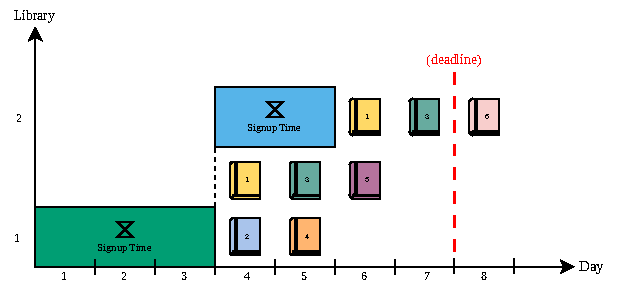
\includegraphics[width=\textwidth,keepaspectratio]{../assets/bs/bs-example.pdf}
  \caption{Book Scanning Process Example}
  \label{fig:bs-example}
\end{figure}

\begin{table}[ht]
  \centering
  \begin{tabular}{cccc}
  \toprule
  Library & Sign-up Time & Rate & Books         \\
  \midrule
  1       & 3            & 2    & 1, 2, 3, 4, 5 \\
  2       & 2            & 1    & 1, 3, 6       \\
  \bottomrule
\end{tabular}
  \caption{Library Properties}
  \label{tab:bs-library-properties}
\end{table}

In this specific example, two libraries have signed up in a non-decreasing order
based on their labels, resulting in a combined sign-up time of 5 days.
Additionally, the scanning rates for these libraries are 2 and 1 for library 1
and 2, respectively. This implies that with this library order, library 1 can
ship a maximum of 8 books, while library 2 can ship 2 books at
most.~Consequently, the latter ends up not contributing one of its books to the
scanning process.~Importantly, this example also highlights a scenario where
both libraries possess duplicate copies of the same books (books 1 and 3).~As
mentioned earlier, these duplicate copies will only be scanned once, regardless
of the number of duplicates, ensuring that they are counted for scoring only
once.

In essence, the objective of this problem is to determine the optimal order for
library sign-ups and book selections for shipping, aiming to maximize the number
of unique books sent for scanning before the deadline. In practical terms, this
translates to maximizing the score awarded by the books that can be scanned.

Mathematically, this can be expressed as shown in~\Cref{eq:objective},
where $\mathcal{B}$ represents the total number of books, $s_{b}$ signifies the
score attributed to scanning book $b$ (for $b = 1, \ldots, \mathcal{B}$), and
$x_{b}$ is a binary variable indicating whether a particular book was shipped
(1) or not (0) by any library.

\begin{equation}
  \label{eq:bs-objective}
  \max{f(s)} = \sum_{b = 1}^{\mathcal{B}}{s_{i} \cdot x_{b}}
\end{equation}

For clarification,~\Cref{ex:bs-problem-scoring} shows an example on how the
objective for this problem is evaluated, given the order for the libraries shown
in~\Cref{fig:bs-example} and the properties exposed in~\Cref{tab:bs-library-properties}.

\begin{example}[Objective Evaluation]
  \label{ex:bs-problem-scoring}
  Consider the books scores presented in~\Cref{tab:bs-example}

  \begin{table}[ht]
    \centering
    \begin{tabular}{ccccccc}
  \toprule
  \textbf{Book}  & 1 & 2 & 3 & 4 & 5 & 6 \\ \midrule
  \textbf{Score} & 3 & 1 & 5 & 4 & 7 & 1 \\
  \bottomrule
\end{tabular}
    \caption{Example Book Scores}
    \label{tab:bs-example}
  \end{table}

  The score obtained for the library scheduling shown in~\Cref{fig:bs-example},
  as determined by the evaluation of the objective~\ref{eq:bs-objective} is~$3 +
    1 + 5 + 4 + 7 = 20$
\end{example}

To conclude, this problem imposes several constraints on various parameters that
describe the book scanning process. The most constraints relevant are shown below:

\begin{description}
  \item[\textbf{$\mathcal{L}$.}] The number of libraries~($ 1 \leq \mathcal{L} \leq 10^5$).
  \item[\textbf{$\mathcal{T}$.}] The number of days required to finish a library sign-up~($ 1 \leq \mathcal{T} \leq 10^5$).
  \item[\textbf{$\mathcal{B}$.}] The number of unique books~($ 1 \leq \mathcal{B} \leq 10^5$).
  \item[\textbf{$\mathcal{N}$.}] The number of books per library~($ 1 \leq \mathcal{N} \leq 10^5$).
  \item[\textbf{$\mathcal{D}$.}] The deadline~($ 0 \leq \mathcal{D} \leq 10^5$).
\end{description}

\section{Model}
\label{sec:odc-model}
In the following, we present the modeling developed for this problem, and
highlight aspects that are relevant for its implementation.

\subsubsection*{Problem}

A problem instance is defined by the set of all libraries available, along with
their sign-up times, book shipping rate, and list of books that can be shipped,
the scores for all the books, and the deadline.

\subsubsection*{Solution}
The solution in this problem is defined by a collection of assignments of books
to libraries and the order in which libraries are scanned. It is important to
note that, in the context of this problem, any partial solution is considered
feasible.

\subsubsection*{Component}

One type of component is a tuple containing a book and library, representing an
assignment. Moreover, given that libraries need to be signed-up in order be
possible to scan books, another type of component is a pair of libraries
$(i, j)$ where, $i = 0, \ldots, \mathcal{L}$ and $j = 1, \ldots, \mathcal{L}$;
denoting that library $j$ is signed-up after library $i$. To denote the first
library that is signed up we consider the component $(0, j)$.


\subsubsection*{Construction Rules}

For this problem, we considered two construction rules which are described as follows:

\paragraph*{Standard}

This approach encompasses enumerating all possible combinations of already
signed-up libraries and not yet scanned books. Additionally, it also enumerates
all libraries that can be signed-up next before the deadline.

\paragraph*{Sequential}

This approach is a slight variation of the previous one. Instead of enumerating
all possible books for all signed-up libraries simultaneously, it only generates
assignments for the last signed-up library and enumerates the books strictly for
that library.~Note that, the selection of which library to sign-up next is also
an enumerated component. As a result, we reduce the complexity of the
enumeration of all components by a factor of~$\mathcal{L}$.

\subsubsection*{Objective Function}

The objective function for this problem is the same as the one defined in the
problem description.

\subsubsection*{Upper Bound}

A possible bound for this problem is to consider each library as a knapsack
problem where the capacity is the number of books that can still be signed-up by
a library until the deadline, and each book represents an item with weight of 1
and profit equal to its score. Note that, for libraries already signed-up the
time until the deadline is known, whereas for libraries that have not yet been
signed up that time is not known. However, we can consider that each not signed
up library will be the next to open, thus relaxing the constraint that dictates
that two libraries can not be signed-up simultaneously. The bound for this
problem is then the sum of a knapsack bound for all libraries considering only
the books that have not yet been signed up and that are available for each
library. Note that, we are also relaxing the fact that each book can only score
once by possibly counting it for the bound of multiple libraries.

Another bound for this problem, is to consider the number of books that can be
shipped until the deadline for all libraries as the knapsack.~Thus, we relax the
constraint set on the number of books that can be scanned for a particular
library imposed by the objective function. Additionally, we consider that a book
can be placed in the knapsack regardless of which library it belongs to. The
association with a specific library is taken into account once the book is
actually scanned. The value of this upper bound is determined by the sum of the
scores of the unique books that can fit within the knapsack.

\subsubsection*{Local Moves}

The local moves considered for this problem include:

\begin{enumerate}
  \item Adding a book to the set of books to be scanned by a given library.
  \item Removing a book from the set of books that were going to be scanned by a
        library.
  \item Swapping books between libraries. This move ensures that both libraries
        have copies of the books being swapped.
  \item Removing a book from the list of books to be scanned by a library and
        adding that book to another library. If possible, replace the removed book in
        the first library with another one that is available there.
\end{enumerate}

\subsubsection*{Perturbation}

Regarding the perturbation of the solution, for this problem, we did not employ
any specific operation apart from randomly applying the described local moves.

\subsection{Two-Phase Approach}

The previous model, although valid, was not competitive in practice. Therefore,
an alternative strategy for modeling this problem was developed. This strategy
involved breaking down the optimization tasks into two distinct stages. The
first stage focused on finding an good order for the libraries, and the second
stage employed an algorithm to assign books to the libraries, effectively
solving the problem.

\subsubsection*{Construction Rules}

The library selection strategy employed was based on a heuristic value
calculated at each step for each library not yet signed-up.~The objective was to
rank the libraries according to their potential contribution given by the books
they contained. There are numerous possible criteria for ranking libraries, such
as prioritizing those with the shortest sign-up time, libraries containing the
rarest books, or libraries with the highest score, among others. However, the
most effective heuristic value for ranking libraries in practice was the one
that takes into account libraries with the highest cumulative score of books not
present in any of the assigned libraries and could be shipped before the
deadline, divided by the sign-up time.

After iteratively selecting libraries based on their heuristic values until it is
no longer possible and defining the library order, we can then solve the book
assignment optimally using an exact method. There are various algorithms in the
literature to solve assignment problems, such as the~\emph{Hungarian
  Method}~\cite{ramshaw2012minimumcost}. However, these algorithms require, in
general, the use of an assignment matrix, which for the instances of this
problem becomes too large and impractical due to memory constraints.

The alternative approach considered involved modeling the problem as a bipartite
graph and using the~\emph{max-flow min-cost} algorithm~\cite{ramshaw2012minimumcost}
to determine the assignment. In this approach, books and libraries were
represented as nodes, and the presence of each book in a library was represented
as an edge. Additionally,~\emph{source} and~\emph{sink} nodes were added to the
graph as required by the algorithm. The bipartite graph is illustrated
in~\Cref{fig:bs-graph}, where there are 3 books and libraries, and book 2 has
duplicate copies in two libraries.

\begin{figure}[h]
  \centering
  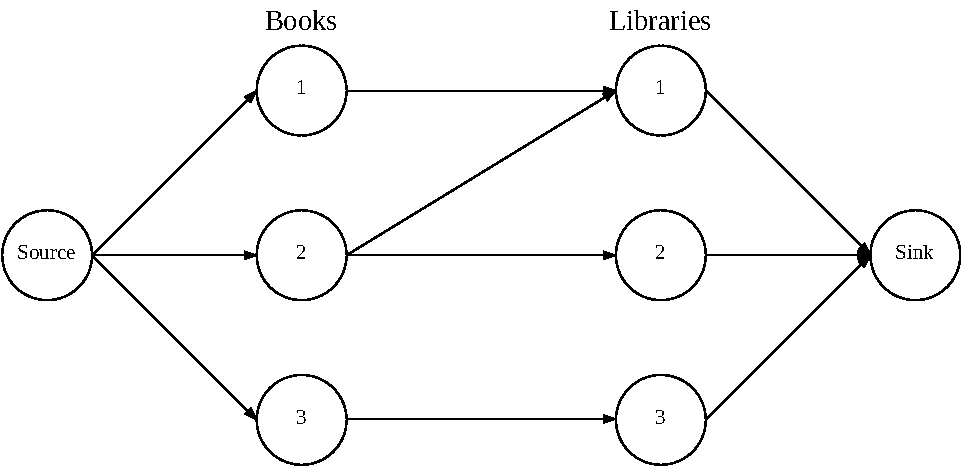
\includegraphics[width=\textwidth,keepaspectratio]{../assets/bs/bs-graph.pdf}
  \caption{Assignment Problem Modeled as a Bipartite Graph}
  \label{fig:bs-graph}
\end{figure}

The edges of the graph are then adjusted in the following way:

\begin{description}
  \item[From \textbf{Source} to \textbf{Books}.] The cost of the edge was set
    to $0$ since we do not wish to count the contribution of this edge, and the capacity
    was set to $1$, symbolizing that all books can be considered for assignment.

  \item[From \textbf{Books} to \textbf{Libraries}.] The cost was set to -$s_{b}$ to
    formulate the problem for maximization, and the capacity was set to $1$, symbolizing
    that each book can be assigned once to that particular library, thereby
    contributing with its score.

  \item[From \textbf{Libraries} to \textbf{Sink}.] The cost was set to $0$
    since libraries do not contribute to the score, and the capacity was given a value
    equal to the number books can be placed in that library, until the deadline~$\mathcal{D}$.
\end{description}

It is important to note that, the assignment will correspond to edges in the
graph that maximize the flow, and secondarily minimize the cost.

\subsubsection*{Local Moves}

To further improve the objective value, we can experiment with different library
orderings by applying the following local moves to the existing order,$\phi^\mathcal{I}$.

\begin{itemize}
  \item Reverse the sign-up order between two libraries in $\phi^\mathcal{I}$
  \item Change the positions of two libraries in the order $\phi^\mathcal{I}$,
        adjusting the sign-up times of every library in between.
  \item Select one library to remove and add another library that is not
        currently considered in that position, if possible.
\end{itemize}

\section{Implementation}
\label{sec:odc-implementation}
\input{mainmatter/5-OptimizeADataCenter/sections/implementation.tex}

\section{Results}
\label{sec:odc-results}
After formally describing the problem model, the information was translated into
a practical implementation developed within the modeling framework mentioned in
Chapter \ref{ch:principled-modelling-framework}. This implementation enabled the
use of various meta-heuristic methods for experimentation. Multiple iterations
of the model were tested, each involving different types of component
enumerations, bounds, heuristics, and various solvers.

The machine used to run the solvers on the single available instance for this
problem had the following s specifications:

\begin{table}[h]
  \centering
  \begin{tabular}{@{\extracolsep{4pt}}ccc@{\extracolsep{4pt}}}
    \toprule
    OS                 & CPU                                     & RAM   \\ \midrule
    Ubuntu 22.04.2 LTS & Intel i7-12700H (20 cores) --- 4.600GHz & 64 GB \\
    \bottomrule
  \end{tabular}
  \caption{Benchmark Machine Specifications}
\end{table}

The best results were achieved through a simple heuristic strategy in a
constructive search phase. This strategy involved enumerating ten first
components at each iteration using the heuristic strategy described
in~\Cref{algorithm:odc-enum-heuristic}. The selected component to add to the
solution was the one that contributed the most increment to the upper bound
value. Notably, the upper bound function used was the one described in Equation
\ref{eq:odc-upper-bound-2}, which effectively discriminated the results,
allowing for a construction that yielded a final score of 386 points in only 1
second.

Other~\acrshort{constructive-search} algorithms, such
as~\acrshort{grasp},~\acrshort{iterated-greedy} and~\acrshort{beam-search}
proved to be slower in constructing solutions of similar quality compared to the
simple heuristic strategy.~Multiple~\emph{add-hoc} parametrizations were tested
for each of these algorithms, but they consistently produced initial results
ranging from 280 to 320 points, taking additional time to further improve them
as to match the described heuristic.

For~\acrshort{local-search} strategy, the best meta-heuristic
was~\acrshort{iterated-local-search}. When run with a total timeout time of 15
seconds and using a perturbation with a kick strength of
2,~\acrshort{iterated-local-search} consistently improved the solution returned
by the heuristic construction strategy (regardless of the seed), yielding a
score of 410 points.~This result was satisfying and led to us move on to the
next problem.

Notably, the score of~\textbf{410} is better than the best score in the
competition leaderboard~(\textbf{407}).

\section{Concluding Remarks}
\label{sec:odc-concluding-remarks}
In this chapter, we conducted a comprehensive exploration of the Google Hash
Code competition, delving into its structure, problem descriptions, and instance
generation. In particular, we established links between the challenges presented
and well-known~\acrshort{combinatorial-optimization} problems. Furthermore, we
highlighted common techniques employed by participants, drawing from our own
engagement in the competition.

We consider this analysis to be an important step that not only facilitated
a deeper comprehension of the challenges, but also guided our choice of two
specific problems (\nameref{subsubsec:hashcode-2015-qualification} and~\nameref{subsubsec:hashcode-2020-qualification}) for detailed
exploration in this study. Thus, in the ensuing chapters, we will discuss our
modeling approach, analyze the chosen problems, and reflect on the conclusions
drawn from the work.






